\documentclass{article}
\usepackage[a4paper, total={6.5in, 10in}]{geometry}
\setlength{\parindent}{0pt}
\usepackage{tcolorbox}
\tcbset{colback=white!94!black, colframe=black!60!white, coltitle = white, boxrule=0.8pt, arc=2mm}
\newtcolorbox{boxs}[2][]{title= #2,#1}
\usepackage{datetime2}
\usepackage{pgfplots}
\usepackage[british]{babel}
\usepackage{amsfonts}
\usepackage{amsmath}
\pgfplotsset{compat=1.18}


\title{\textbf{Polar Coordinates}}
\author{Robert O'Connell}
\date{\today}

\usepackage{tikz}
\usepackage{amsmath}
\usetikzlibrary{arrows.meta,angles,quotes}

\begin{document}
\maketitle
\subsection*{Example Plot}
\begin{center}
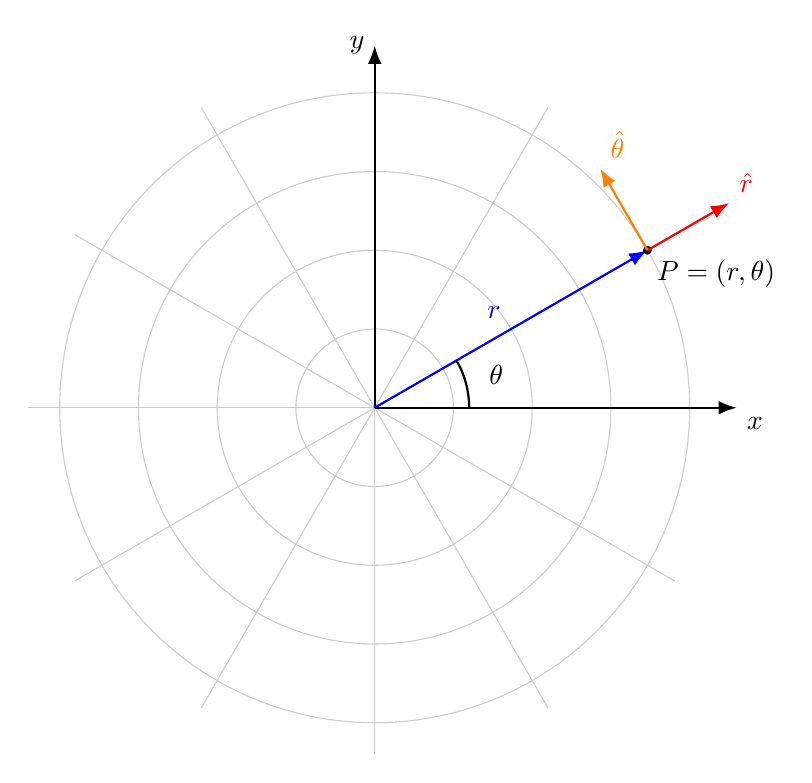
\begin{tikzpicture}[scale=2, >=Latex]

% --- PARAMETERS ---
\def\r{2}   % radius of point
\def\th{30} % angle in degrees
\def\len{0.6} % length of unit vectors

% --- POLAR GRID ---
% Circular grid lines
\foreach \rad in {0.5,1,1.5,2} {
  \draw[gray!40] (0,0) circle (\rad);
}
% Radial lines every 30 degrees
\foreach \ang in {0,30,...,330} {
  \draw[gray!40] (0,0) -- ({2.2*cos(\ang)},{2.2*sin(\ang)});
}

% --- AXES ---
\draw[->,thick] (0,0) -- (2.3,0) node[below right] {$x$};
\draw[->,thick] (0,0) -- (0,2.3) node[left] {$y$};

% --- RADIAL VECTOR r ---
\draw[->,thick,blue] (0,0) -- ({\r*cos(\th)},{\r*sin(\th)})
  node[midway,above left] {$r$};
\fill ({\r*cos(\th)},{\r*sin(\th)}) circle (0.8pt)
  node[below right] {$P = (r,\theta)$};

% --- ANGLE ARC ---
\draw[thick] (0.6,0) arc[start angle=0,end angle=\th,radius=0.6];
\node at ({0.8*cos(\th/2)},{0.8*sin(\th/2)}) {$\theta$};

% --- UNIT VECTORS ---
\draw[->,red,thick] ({\r*cos(\th)},{\r*sin(\th)}) --
  ++({\len*cos(\th)},{\len*sin(\th)}) node[above right] {$\hat{r}$};
\draw[->,orange,thick] ({\r*cos(\th)},{\r*sin(\th)}) --
  ++({-\len*sin(\th)},{\len*cos(\th)}) node[above right] {$\hat{\theta}$};

\end{tikzpicture}
\end{center}

From the plot we can see that
\[
r = \sqrt{x^2+y^2}
\]
\[
\theta = \tan^{-1}\left(\frac{y}{x}\right)
\]

\subsection*{Basis Vectors (\(\hat{r}, \hat{\theta}\))}
The basis vectors \(\hat{r}\) and \(\hat{\theta}\) rotate as \(\theta\) changes

\(\hat{r}\) points radially outward from the origin, while \(\hat{\theta}\) is tagent to the circle in the direction of increasing \(\theta\)

And,
\[
\hat{r} \cdot \hat{\theta} = 0
\]
\[
\Rightarrow \hat{r} \perp \hat{\theta}
\]

Defining (\(\hat{r}, \hat{\theta}\)) from cartesian basis vectors
\[
\hat{r} = \cos(\theta) \hat{i} + \sin(\theta)\hat{j}
\]
\begin{align*}
    \hat{\theta} &= -\cos(\frac{\pi}{2}- \theta)\hat{i} + \sin(\frac{\pi}{2} -\theta)\hat{j} \\
    &= -\sin(\theta) \hat{i} + \cos(\theta) \hat{j}
\end{align*}

\newpage
\subsection*{Position, Velocity and Acceleration Derivatives}
\begin{align*}
    \vec{r}(t) &= r\cos(\theta)\hat{i} + r\sin(\theta)\hat{j} \\
    &= r\hat{r}
\end{align*}

\begin{align*}
    \vec{v}(t) &= \frac{d}{dt}(r\hat{r}) \\
    &= \frac{dr}{dt}\hat{r} + r \frac{d\hat{r}}{dt} \\
    \frac{d\hat{r}}{dt} = -\sin(\theta) \frac{d\theta}{dt} \hat{i} &+ \cos(\theta) \frac{d\theta}{dt} \hat{j} = \frac{d\theta}{dt}\hat{\theta} \\
    \\
    \Rightarrow \vec{v}(t)&= \dot{r}\hat{r} + r\dot{\theta}\hat{\theta}
\end{align*}
The velocity has two components, one along \(\hat{r}\) (changing the distance from the origin) and one along \(\hat{\theta}\) (changing the angle)

\begin{align*}
    \vec{a}(t) &= \frac{d}{dt} (\dot{r}\hat{r} + r\dot{\theta}\hat{\theta}) \\
    &= \ddot{r}\hat{r} + \dot{r}\frac{d\hat{r}}{dt} + \dot{r}\dot{\theta}\hat{\theta} + r\dot{\theta}\frac{d\hat{\theta}}{dt} \\
    \frac{d\hat{\theta}}{dt} = \frac{d}{dt}(&-\sin(\theta) \hat{i} + \cos(\theta) \hat{j}) = -\dot{\theta}\hat{r} \\
    \\
    \Rightarrow \vec{a}(t)&=(\ddot{r}-r\dot{\theta}^2)\hat{r} + (2\dot{r}\dot{\theta}+ r \ddot{\theta})\hat{\theta} 
\end{align*}

The first term, $(\ddot{r} - r\dot{\theta}^2)\hat{r}$, represents the
radial acceleration. The negative component $-r\dot{\theta}^2\hat{r}$ corresponds
to the centripetal acceleration directed toward the origin.

The second term, $(2\dot{r}\dot{\theta} + r\ddot{\theta})\hat{\theta}$, represents
the tangential acceleration. Here, $2\dot{r}\dot{\theta}\hat{\theta}$ is the Coriolis component,
and $r\ddot{\theta}\hat{\theta}$ arises from angular acceleration.
\end{document}
